\documentclass{beamer}

\usepackage{beamerthemesplit}
\usepackage{verbatim}

\usepackage{xcolor}

\definecolor{gold}{rgb}{1.,0.84,0.}
\definecolor{brightred}{rgb}{1.,0.4,0.4}
\definecolor{mygray}{RGB}{200,200,200}
\definecolor{lightsteelblue}{RGB}{176,196,222}
\definecolor{lightskyblue}{RGB}{135,206,250}
\definecolor{cadetblue}{RGB}{95,158,160}

\usetheme{default}
\usecolortheme{mule}

\usefonttheme{serif}

%\DeclareGraphicsExtensions{.pdf,.png,.jpg}


\newcommand{\mcal}{metacalibration}
\newcommand{\Mcal}{Metacalibration}

\newcommand{\prelim}{{\bf{\it Preliminary}}}



\title{Metacalibration for Weak Lensing Shear Measurement}
\author{Erin Sheldon}
\institute{Brookhaven National Laboratory\\LSST DESC Meeting at SLAC}

% http://texblog.net/latex-archive/plaintex/beamer-footline-frame-number/
% to add the page (frame ) number and not screw up the bottom line
% works for split themes?
\expandafter\def\expandafter\insertshorttitle\expandafter{%
      \insertshorttitle\hfill%
        \insertframenumber\,/\,\inserttotalframenumber}

% suppress navigation bar
\beamertemplatenavigationsymbolsempty
\setbeamertemplate{footline}{}

\begin{document}

\frame{\titlepage}


\setbeamertemplate{background canvas}[vertical shading][bottom=mgray,top=mblack]

\frame
{
    \frametitle{Outline}

    \setbeamerfont*{itemize/enumerate body}{size=\Large}
    \setbeamerfont*{itemize/enumerate subbody}{parent=itemize/enumerate body}
    \setbeamerfont*{itemize/enumerate subsubbody}{parent=itemize/enumerate body}
 
    \begin{itemize}

        %\item The Primary Goal is to Study Dark Energy
        \item Metacalibration

            \begin{itemize}
                \item Correction for Correlated Noise

                \item Performance on Very Large Simulations
            \end{itemize}

    \end{itemize}

}

\frame
{
    \frametitle{Shear Accuracy Requirements}

    \setbeamerfont*{itemize/enumerate body}{size=\Large}
    \setbeamerfont*{itemize/enumerate subbody}{parent=itemize/enumerate body}
    \setbeamerfont*{itemize/enumerate subsubbody}{parent=itemize/enumerate body}
 
    \begin{itemize}

        \item In order to measure the properties of Dark Energy to our desired
            precision, we must measure shear with exquisite accuracy.

            \begin{itemize}
                \item Shear calibration errors: {\color{brightred} $\Delta \gamma/\gamma \lesssim 10^{-3}$}
                \item Additive errors: {\color{brightred} $\Delta \gamma \lesssim 2 \times 10^{-4}$}
            \end{itemize}
    \end{itemize}

}



\frame
{
    \frametitle{Metacalibration Idea from Eric Huff}

    \setbeamerfont*{itemize/enumerate body}{size=\Large}
    \setbeamerfont*{itemize/enumerate subbody}{parent=itemize/enumerate body}
    \setbeamerfont*{itemize/enumerate subsubbody}{parent=itemize/enumerate body}
 

    {\Large
        \begin{itemize}
            \item Say we have a biased shear point estimator {\color{gold} $E$}.  We can write a taylor expansion
                {\color{mygray}
                    \begin{eqnarray}
                        E & = & E(\gamma=0) + \gamma \frac{\partial E}{\partial \gamma} \bigg|_{\gamma=0} + ... \nonumber \\
                          & \sim &  \gamma \frac{\partial E}{\partial \gamma}\bigg|_{\gamma=0}  \equiv \gamma R \nonumber 
                    \end{eqnarray}
                } 
            \item {\color{gold} $R$} is the {\em response} of the estimator $E$ to a shear.
            \item Can write a similar response to the PSF shape $R^p$.
        \end{itemize}
    }
}

\frame
{
    \frametitle{Metacalibration Idea from Eric Huff}

    \setbeamerfont*{itemize/enumerate body}{size=\large}
    \setbeamerfont*{itemize/enumerate subbody}{parent=itemize/enumerate body}
    \setbeamerfont*{itemize/enumerate subsubbody}{parent=itemize/enumerate body}

    \begin{itemize}

        \item Use image manipulation to estimate the derivative of the
            estimator with respect to shear
            {\color{gold}
                \begin{equation}
                    R = \frac{E(+\gamma) - E(-\gamma)}{2 \gamma} \nonumber 
                \end{equation}
            }
            \begin{itemize}
                \item Deconvolve the PSF
                \item Shear the image by a small amount
                \item Reconvolve by the PSF.  Use a slightly larger PSF to suppress
                    the noise amplification
            \end{itemize}

            \item These operations can be done with GALSIM
            \item Insensitive to applied shear $\gamma$.  {\color{lightskyblue} No tunable parameters}


    \end{itemize}

}

\frame
{
    \frametitle{Metacalibration Idea from Eric Huff}

    \setbeamerfont*{itemize/enumerate body}{size=\Large}
    \setbeamerfont*{itemize/enumerate subbody}{parent=itemize/enumerate body}
    \setbeamerfont*{itemize/enumerate subsubbody}{parent=itemize/enumerate body}
 
    \begin{itemize}
        \item Final estimator
            \begin{equation}
                \gamma = \frac{\langle E \rangle - \langle E^p \rangle \langle R^p \rangle }{ \langle R \rangle} \nonumber
            \end{equation}
       

        \item Corrects for {\color{lightskyblue} model bias}

        \item Corrects for {\em ordinary} {\color{gold} noise bias}

        \item Works well at {\color{lightsteelblue} high shear $\gamma \sim 0.08$}

        \item (Huff \& Mandelbaum use a more complex estimator to deal with noisy
            $R$ for regauss)

    \end{itemize}

}

\frame
{
    \frametitle{Correlated Noise}
 
    \begin{center}
        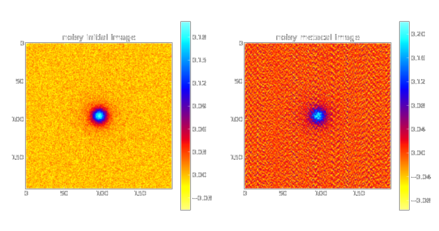
\includegraphics[scale=1]{metacal_noise_images_neg_crop.png}
        \newline
    \end{center}
    {\small Image: Eric Huff}

}



\frame
{
    \frametitle{Correlated Noise}

    \setbeamerfont*{itemize/enumerate body}{size=\large}
    \setbeamerfont*{itemize/enumerate subbody}{parent=itemize/enumerate body}
    \setbeamerfont*{itemize/enumerate subsubbody}{parent=itemize/enumerate body}
 
    \begin{itemize}

        \item These convolutions and shears result in {\em {\color{brightred} correlated noise}}
            
        \begin{itemize}
            \item After convolution, fluctuations due to noise are no longer
                independent between pixels

            \item Shearing involves interpolation, so in a similar way fluctuations
                due to noise are no longer independent
        \end{itemize}

    \item Effect goes as {\color{orange} square} of the noise (Hirata 2016, in prep)

        \item Results from Huff \& Mandelbaum on GREAT3 affected little, as
            $S/N \gtrsim 20$ in that sim.

        \item I found bias of order 10\% for galaxies at $S/N \sim 10$.



    \end{itemize}

}


%\frame
%{
%    \frametitle{Correlated Noise}
%    \begin{itemize}
%
%        \item Approximately cancels from mean estimator
%            {\color{lightskyblue}
%                \begin{equation}
%                    E = \frac{E(+\Delta \gamma) + E(-\Delta\gamma)}{2} \nonumber
%                \end{equation}
%            }
%
%        \item Does not cancel from the response $R$
%            {\color{gold}
%                \begin{equation}
%                    R = \frac{E(+\Delta\gamma) - E(-\Delta\gamma)}{2 \Delta \gamma} \nonumber 
%                \end{equation}
%            }
%
%    \end{itemize}
%
%}


\frame
{
    \frametitle{Correction for Correlated Noise}

    \setbeamerfont*{itemize/enumerate body}{size=\large}
    \setbeamerfont*{itemize/enumerate subbody}{parent=itemize/enumerate body}
    \setbeamerfont*{itemize/enumerate subsubbody}{parent=itemize/enumerate body}
 
    \begin{itemize}

        \item Best correction involves adding {\color{lightskyblue} extra noise}.

        \item Run the image through the \mcal\ procedure with
            shear $\gamma$.

        \item Create a noise field, run through the same \mcal\ steps but with
            the {\color{lightskyblue} opposite shear} $-\gamma$.

        \item Add this noise image to cancel the effect

    \end{itemize}

}



%\frame
%{
%    \frametitle{Detrending Correction for Correlated Noise}

%    {\color{gold} $\Delta R_{\mathrm{noise}} = A \Delta n^2$ } where $\Delta R$
%    is {\color{gold} $R (\mathrm{noise~added~before}) - R(\mathrm{noise~added~after})$ }

%    \begin{figure}
%        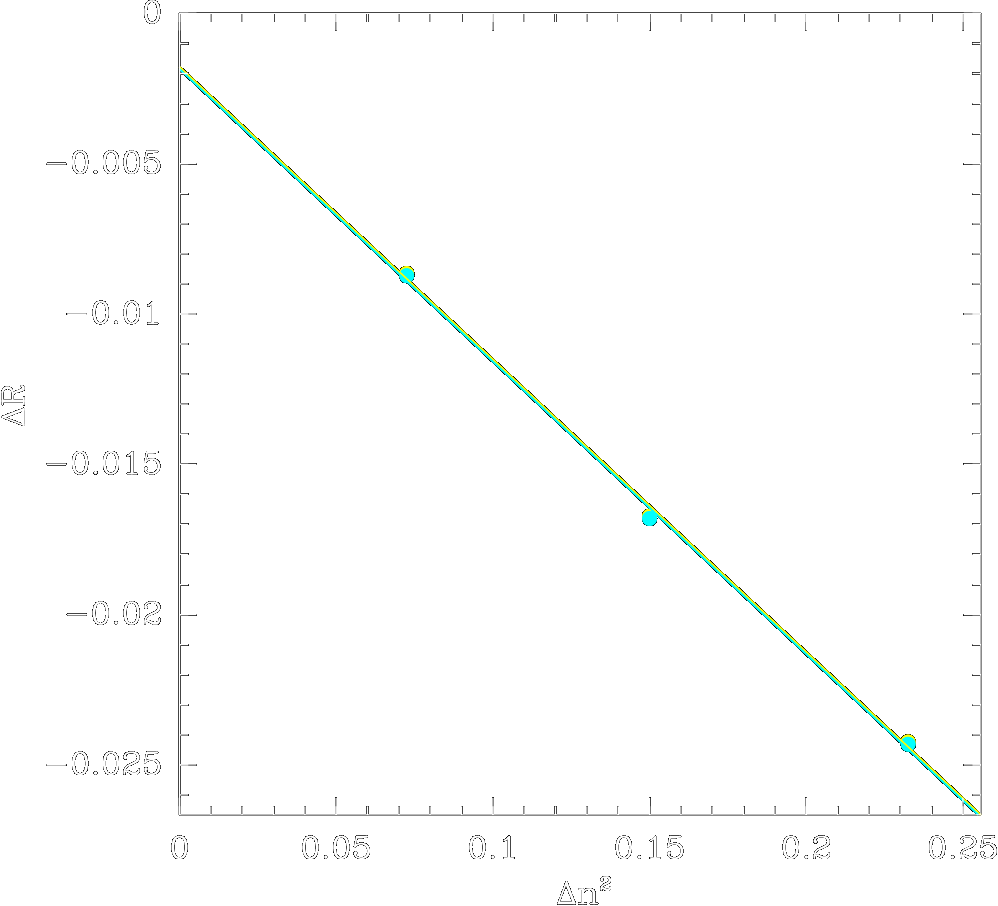
\includegraphics[width=0.6\textwidth]{run-bd13mcal-dt01-Rnoise-detrend-neg.png}
%    \end{figure}

%    Note offset is not zero.  Use 
%    {\color{lightskyblue} $R_{\mathrm{noise}} = A n^2 - \mathrm{offset}$}
%}

\frame
{
    \frametitle{COSMOS Simulations}

    \setbeamerfont*{itemize/enumerate body}{size=\large}
    \setbeamerfont*{itemize/enumerate subbody}{parent=itemize/enumerate body}
    \setbeamerfont*{itemize/enumerate subsubbody}{parent=itemize/enumerate body}
 
    \begin{itemize}
        \item Similar to {\color{lightskyblue} GREAT3 RGC}

        \item COSMOS galaxies sheared; smeared by PSF

        \item Optical model from DES (Aaron Roodman), plus Kolmogrov atmosphere
        \item {\color{gold} No ring} configuration
        \item Mode of {\color{orange} $S/N \sim 10$}
        \item $10^8$ galaxies

        \item {\color{gold} \texttt{egret}} code from Matt Becker, fork of \texttt{great3-public} repo
            https://github.com/esheldon/egret

    \end{itemize}

}

\frame
{
    \frametitle{Parametric Simulations}

    \setbeamerfont*{itemize/enumerate body}{size=\large}
    \setbeamerfont*{itemize/enumerate subbody}{parent=itemize/enumerate body}
    \setbeamerfont*{itemize/enumerate subsubbody}{parent=itemize/enumerate body}
 
    \begin{itemize}

        \item {\color{gold} Bulge+Disk}

        \item Half-light radius distribution matched to COSMOS

        \item Large offsets between bulge and disk centers:
            {\color{lightskyblue} not described by an ellipse}.

        \item Moffat PSF with size and shape distribution
            matched to DES.  PSF $e_2$ not round on average.

        \item Signal-to-noise ratio distribution matched to real DES
            data, with {\color{lightskyblue} mode $S/N \sim$10}.  Induces ordinary noise
            bias of order 10\%
        
        \item Include 10\% {\color{brightred} stars} and realistic pixel
            {\color{orange} masking} from DES

        \item $2 \times 10^8$ galaxies


    \end{itemize}

}

\frame
{
    \frametitle{Parametric Simulations}
 
    \begin{center}
        
\includegraphics[width=0.8\textwidth]{s2n-bd16-icolor.pdf}
    \end{center}

}


\frame
{
    \frametitle{Performance on Simulations: Fitting}

    \setbeamerfont*{itemize/enumerate body}{size=\large}
    \setbeamerfont*{itemize/enumerate subbody}{parent=itemize/enumerate body}
    \setbeamerfont*{itemize/enumerate subsubbody}{parent=itemize/enumerate body}
 
    \begin{itemize}
        \item Intentionally fit {\color{brightred} terrible models}.

        \item Fit single Gaussian to PSF: large errors in
            PSF correction.

        \item Fit a single Gaussian to galaxy: large ``model bias''.

        \begin{itemize}
            \item Apply strong prior on the shape: good for stability but
                introduces a large shear bias
        \end{itemize}
        \item Low S/N means lots of noise bias.

        ~
        \item Correct for these with \mcal.

        ~
        \item Model the bias as a multiplicative and an additive part
            {\color{lightskyblue} 
                \begin{equation}
                    \gamma = (1 + m ) \times \gamma_{true} + c \nonumber
                \end{equation}
            }

    \end{itemize}
}

\frame
{
    \frametitle{Performance on Simulations: COSMOS Sims}

    \setbeamerfont*{itemize/enumerate body}{size=\large}
    \setbeamerfont*{itemize/enumerate subbody}{parent=itemize/enumerate body}
    \setbeamerfont*{itemize/enumerate subsubbody}{parent=itemize/enumerate body}
 
    \begin{itemize}
            
            

         \item COSMOS simulations with real galaxies and DES optical model.

        \item Maximum Likelihood 
            {\color{brightred} 
                \begin{eqnarray}
                    m & = & -0.4  \nonumber \\
                  c_1 & = & (-0.2 \pm 0.2) \times 10^{-4} \nonumber \\
                  c_2 & = & (+0.3 \pm 0.2) \times 10^{-4} \nonumber
                \end{eqnarray}
            }


         \item Using \mcal:
        {\color{gold} 
            \begin{eqnarray}
                %m & = & (+0.5 \pm 0.6) \times 10^{-3} \nonumber \\
                m & = & (5 \pm 6) \times 10^{-4} \nonumber \\
              c_1 & = & (-0.4 \pm 0.3) \times 10^{-4} \nonumber \\
              c_2 & = & (+0.6 \pm 0.3) \times 10^{-4} \nonumber
            \end{eqnarray}
        }
         \item No detected bias at the level required for LSST.
    \end{itemize}

}

\frame
{
    \frametitle{Performance on Simulations}
 
    {\normalsize Maximum Likelihood}
    \begin{center}
        
\includegraphics[width=0.65\textwidth]{run-bd29mcal01-fit-m-c-nocorr-icolor.pdf}
    \end{center}

    {\normalsize Metacalibration}
    \begin{center}
        
\includegraphics[width=0.65\textwidth]{run-bd29mcal01-fit-m-c-icolor.pdf}
    \end{center}

}




\frame
{
    \frametitle{Performance on Parametric Simulations}

    \setbeamerfont*{itemize/enumerate body}{size=\large}
    \setbeamerfont*{itemize/enumerate subbody}{parent=itemize/enumerate body}
    \setbeamerfont*{itemize/enumerate subsubbody}{parent=itemize/enumerate body}
 
    \begin{itemize}


        \item Maximum Likelihood 
            {\color{brightred} 
                \begin{eqnarray}
                    m & = & -0.5  \nonumber \\
                  c_1 & = & (+0.1 \pm 0.1) \times 10^{-4} \nonumber \\
                  c_2 & = & (+15.1 \pm 0.1) \times 10^{-4} \nonumber
                \end{eqnarray}
            }


        \item Using \mcal:

            {\color{gold} 
                \begin{eqnarray}
                    m & = & (-4 \pm 5) \times 10^{-4} \nonumber \\
                  c_1 & = & (+0.0 \pm 0.2) \times 10^{-4} \nonumber \\
                  c_2 & = & (+0.9 \pm 0.2) \times 10^{-4} \nonumber
                \end{eqnarray}
            }
            %{\color{gold} 
            %    \begin{eqnarray}
            %        m & = & (-0.4 \pm 0.5) \times 10^{-3} \nonumber \\
            %      c_1 & = & (+0.0 \pm 0.2) \times 10^{-4} \nonumber \\
            %      c_2 & = & (+0.9 \pm 0.2) \times 10^{-4} \nonumber
            %    \end{eqnarray}
            %}


        \item No detected multiplicative bias.
        \item Some remaining PSF leakage: Just use
            better PSF correction than a Gaussian!

    \end{itemize}

}


\frame
{
    \frametitle{Performance on Simulations: Stars}
 
    \begin{center}
        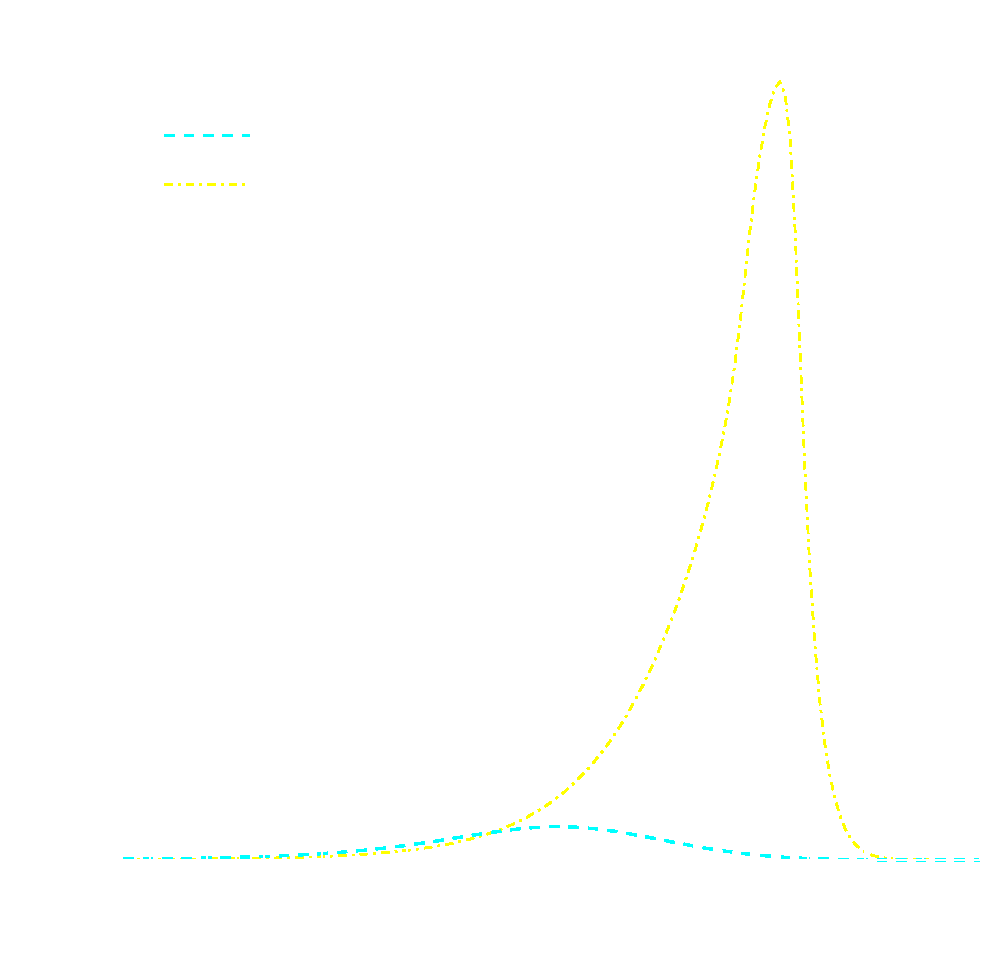
\includegraphics[width=0.7\textwidth]{R-dt-with-stars-icolor.pdf}
        \newline
        {\large Response for stars and galaxies}
    \end{center}

}



\frame
{
    \frametitle{Performance on Simulations: Stars}

    \setbeamerfont*{itemize/enumerate body}{size=\large}
    \setbeamerfont*{itemize/enumerate subbody}{parent=itemize/enumerate body}
    \setbeamerfont*{itemize/enumerate subsubbody}{parent=itemize/enumerate body}
 
    \begin{itemize}

        \item Parametric simulation with and without {\color{gold} 10\% stars}
             {\color{lightskyblue} 
                 \begin{eqnarray}
                     %m        & = & (+0.5 \pm 0.4) \times 10^{-3} \nonumber \\
                     %m(stars) & = & (+0.5 \pm 0.5) \times 10^{-3} \nonumber
                     m        & = & (5 \pm 4) \times 10^{-4} \nonumber \\
                     m(stars) & = & (5 \pm 5) \times 10^{-4} \nonumber
                 \end{eqnarray}
             }

         \item Including stars introduces additional noise, but no
             additional bias: In the mean, stars have zero response {\color{gold} $R$}.

             {\color{mygray} 
                 \begin{equation}
                     \gamma = \frac{\sum e_{gals} + \sum e_{stars}}{\sum R_{gals} + \sum R_{star}} \nonumber
                 \end{equation}
             }


    \end{itemize}

}



\frame
{
    \frametitle{Performance on Simulations}

    \setbeamerfont*{itemize/enumerate body}{size=\large}
    \setbeamerfont*{itemize/enumerate subbody}{parent=itemize/enumerate body}
    \setbeamerfont*{itemize/enumerate subsubbody}{parent=itemize/enumerate body}
 
    \begin{itemize}
            

        \item Parametric simulations with {\color{brightred} masking based on DES}
         \item Replace masked pixels with the best fit model

             {\color{lightsteelblue} 
                 \begin{eqnarray}
                     %m & = & (-0.5 \pm 0.3) \times 10^{-3} \nonumber \\
                     m & = & (-5 \pm 3) \times 10^{-4} \nonumber \\
                   c_1 & = & (+0.0 \pm 0.2) \times 10^{-4} \nonumber \\
                   c_2 & = & (+1.1 \pm 0.2) \times 10^{-4} \nonumber
                 \end{eqnarray}
             }

         \item FFTs not biased by replacing masked pixels with model

    \end{itemize}

}


\frame
{
    \frametitle{Future Work}

    \setbeamerfont*{itemize/enumerate body}{size=\Large}
    \setbeamerfont*{itemize/enumerate subbody}{parent=itemize/enumerate body}
    \setbeamerfont*{itemize/enumerate subsubbody}{parent=itemize/enumerate body}
 
    \begin{itemize}
            

         \item Selection Effects:
             \begin{itemize}
                 \item Detection effects:  Requires prior information.
                 \item Ordinary selections.  
             \end{itemize}

         \item Variable shear inference

    \end{itemize}

}



\frame
{
    \frametitle{Summary}

    \setbeamerfont*{itemize/enumerate body}{size=\Large}
    \setbeamerfont*{itemize/enumerate subbody}{parent=itemize/enumerate body}
    \setbeamerfont*{itemize/enumerate subsubbody}{parent=itemize/enumerate body}
 
    \begin{itemize}
        \item Metacalibration is a new idea for shear recovery from
            Eric Huff

        \item No tunable parameters.

        \item Straightforward correction for correlated noise.

        \item Bias on simulations is within LSST requirements.
        
    \end{itemize}

}

\end{document}
